\begin{thm}{200}{\hosi 10\maru}{DMO4th 理4}
 正の整数$n$と実数$a$に対して、関数$I_n(a)$を、
 \[ I_n(a)=\int_0^{\frac{\pi}{2}}\! \left|\cos^n x-a\sin^n2x\right| \,dx \]
 で定め、$m_n$を$I_n(a)$の最小値とする。$m_n$の最大値を求めよ。
\end{thm}

$a\le\dfrac{1}{2^n}$のとき、
\[ \cos^n x-a\sin^n 2x=\cos^n x\left(1-2^na\sin^n x\right) \]
は、$2^n a\sin^n x \le 2^n\cdot\dfrac{1}{2^n}\cdot 1=1$から非負であるから、
\[ I_n(a)=\int_0^{\frac{\pi}{2}}\! \cos^n x \,dx -a\left(\int_0^{\frac{\pi}{2}}\! \sin^n 2x \,dx\right) \]
は$a$についての1次関数である。$0\le x\le\dfrac{\pi}{2}$で$\sin^n 2x$は常に0以上の値をとるから、$I_n(a)$は単調減少し、$I_n(a)\ge I_n\left(\dfrac{1}{2^n}\right)$。

$a>\dfrac{1}{2^n}$のとき、$0<x<\dfrac{\pi}{2}$で$\cos^n x\neq 0$、$1-2^na\sin^n x$は単調減少する。また、
\[ 1-2^na\sin^n 0=1>0, \qquad 1-2^nasin^n\frac{\pi}{2}=1-2^na<0 \]
となるので、$\cos^n p(1-2^na\sin^n p)=0$~($\cdots$ *)を満たす実数$p$~($0<p<\dfrac{\pi}{2}$) がただひとつ存在する。この$p$を用いて、
\[ I_n(a)=\int_0^p\!(\cos^n x-a\sin^n 2x) \,dx+\int_p^{\frac{\pi}{2}}\!(a\sin^n 2x-\cos^n x) \,dx \]
となり、$\cos^n x$, $\sin^2 2x$の原始関数の1つを$F(x)$, $G(x)$とすると、$I_n(a)$は以下のように求められる。
\begin{align*}
 I_n(a)&=\Bigl[F(x)-aG(x)\Bigr]_0^p+\Bigl[aG(x)-F(x)\Bigr]_p^{\frac{\pi}{2}} \\
 &=2F(p)-2aG(p) \\
 &\qquad +a\left[G(0)+G\left(\frac{\pi}{2}\right)\right]-\left[F(0)+F\left(\frac{\pi}{2}\right)\right]
\end{align*}

これを$a$で微分すると、
\begin{align*}
 \frac{d}{da}I_n(a)&=2\frac{dp}{da}\frac{d}{dp}F(p)-2\left(G(p)-a\frac{dp}{da}\frac{d}{dp}G(p)\right) \\
 &\qquad +\left(G(0)+G\left(\frac{\pi}{2}\right)\right) \\
 &=2\frac{dp}{da}\left(\cos^n p-a\sin^n 2p\right) + G(0)-2G(p)+G\left(\frac{\pi}{2}\right) \\
 &=G(0)-2G(p)+G\left(\frac{\pi}{2}\right) \qquad (\because \text{*}) \\
 &=\int_p^{\frac{\pi}{2}}\!\sin^n 2x \,dx -\int_0^p\! \sin^n 2x \,dx
\end{align*}
\begin{wrapfigure}[7]{r}[0pt]{150pt}
 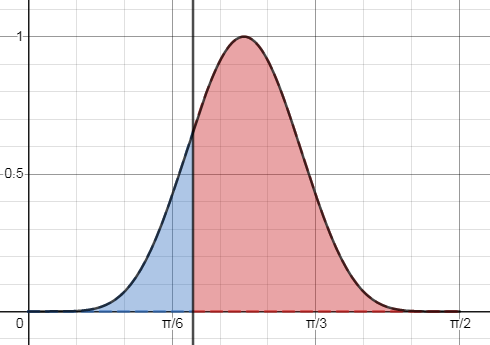
\includegraphics[width=\linewidth]{../problems/Q_200/A_200_1.png}
\end{wrapfigure}
この積分は、右図の面積における$(\text{赤領域})-(\text{青領域})$であることから、$p=\dfrac{\pi}{4}$で$\dfrac{d}{da}I_n(a)=0$となり、$0<p<\dfrac{\pi}{4}$で$\dfrac{d}{da}I_n(a)<0$、$\dfrac{\pi}{4}<p<\dfrac{\pi}{2}$で$\dfrac{d}{da}I_n(a)>0$となる。したがって、$p=\dfrac{\pi}{4}$となる$a$で、$I_n(a)$は極小値をとる。(*)によって、$a=\dfrac{1}{2^n\sin^n p}$なので、このときの$a$は$a=\dfrac{1}{\sqrt{2}^n}$。

%\begin{figure}[H]
% \centering
% 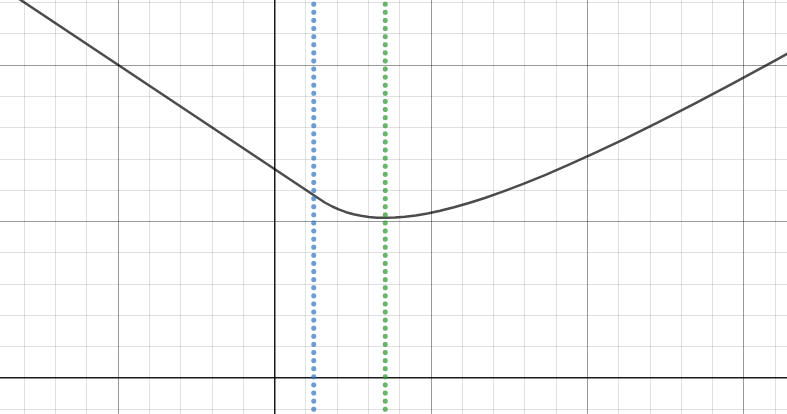
\includegraphics[width=0.7\linewidth]{../problems/Q_200/A_200_2.png}
%\end{figure}
以上のことから、$I_n\left(\frac{1}{2^n}\right)>I_n\left(\frac{1}{\sqrt{2}^n}\right)$がわかるので、$m_n=I_n\left(\dfrac{1}{\sqrt{2}^n}\right)$であり、このとき$p=\dfrac{\pi}{4}$だから、
\[ m_n=\int_0^{\frac{\pi}{4}}\!(\cos^n x-a\sin^n 2x) \,dx + \int_{\frac{\pi}{4}}^{\frac{\pi}{2}}\!(a\sin^n 2x-\cos^n x) \,dx \]
となる。第2項において、$x=\dfrac{\pi}{2}-t$と置換すれば、
\[ m_n=\int_0^{\frac{\pi}{4}}\!(\cos^n x-a\sin^n 2x) \,dx + \int_{\frac{\pi}{4}}^0\!(a\sin^n 2t-\cos^n t) \,(-dt) \]
さらに整理して以下を得る。
\[ m_n=\int_0^{\frac{\pi}{4}}(\cos^n x-\sin^n x) \,dx \]
$n\ge 3$のとき、
\begin{align*}
 m_n&=\int_0^{\frac{\pi}{4}}\!(\cos^n x-\sin^n x)(\cos^2 x+\sin^2 x)\,dx \\
 &=\int_0^{\frac{\pi}{4}}\! (\cos^{n+2}x -\sin^{n+2}x) \,dx \\
 &\qquad + \int_0^{\frac{\pi}{4}}\!\sin^2\cos^2x(\cos^{n-2}x-\sin^{n-2}x)\,dx \\
 &> \int_0^{\frac{\pi}{4}}\!(\cos^{n+2}x-\sin^{n+2}x) \,dx = m_{n+2} \quad (\because \text{第2項は正})
\end{align*}
によって、$m_3>m_5>m_7>\dots$,~$m_4>m_6>m_8>\dots$ となる。よって$m_n$が最大となるのは$n=1, 2, 3, 4$のいずれか。
\begin{align*}
 m_1&=\int_0^{\frac{\pi}{4}}\!(\cos x-\sin x) \,dx = \Bigl[\sin x+\cos x\Bigr]_0^{\frac{\pi}{4}}=\sqrt{2}-1 \\
 m_2&=\int_0^{\frac{\pi}{4}}\!(\cos^2x-\sin^2x) \,dx \\
 &=\int_0^{\frac{\pi}{4}}\! \cos 2x \,dx=\Bigl[\frac{1}{2}\sin 2x\Bigr]_0^{\frac{\pi}{4}}=\frac{1}{2} \\
 m_3&=\int_0^{\frac{\pi}{4}}\!(\cos^3x-\sin^3x) \,dx \\
 &= \int_0^{\frac{\pi}{4}}\!\cos x(1-\sin^2 x) \,dx-\int_0^{\frac{\pi}{4}}\!\sin x(1-\cos^2 x) \,dx \\
 &=\int_0^{\frac{\pi}{4}}\!(\cos x-\sin x)\,dx+\int_0^{\frac{\pi}{4}}\!(\cos^2 x\sin x-\cos x\sin^2 x) \,dx \\
 &= m_1+\Bigl[-\frac{1}{3}\cos^3 x-\frac{1}{3}\sin^3 x\Bigr]_0^{\frac{\pi}{4}} = \frac{5\sqrt{2}-4}{6} \\
 m_4&=m_2-\int_0^{\frac{\pi}{4}}\!\sin^2 x\cos^2 x(\cos^0 x-\sin^0 x) \,dx = m_2 = \frac{1}{2}
\end{align*}
これらについて、$7<5\sqrt{2}<8$であることに注意して、
\begin{align*}
 m_3-m_1&=\frac{2-\sqrt{2}}{6}>0 \\
 m_3&=\frac{5\sqrt{2}-4}{6}>\frac{7-4}{6}=\frac{1}{2}=m_2=m_4
\end{align*}
がわかるので、$m_n$の最大値は$n=3$のとき\footnote{$n$を実数にまで広げれば、$n=2\sqrt{2}$のときに$m_n$は最大となる(未証明 by math\_Hurdia)}で、$\dfrac{5\sqrt{2}-4}{6}$